\documentclass[leqno,twocolumn]{article}
\usepackage[margin=0.5in]{geometry}
\usepackage[utf8]{inputenc}
\usepackage{amsmath, amsfonts, color, booktabs, centernot, graphicx, fancyhdr}
\usepackage[linktoc=all,hidelinks]{hyperref}
\setlength\parindent{0pt}
\begin{document}
\onecolumn
\title{Journal of Spring 2015}
\author{Leah Dickstein}

\maketitle

\tableofcontents

\section{Adding Quantization Noise: Theoretical}
\subsection{Model of Summer 2014:}
\[ X(n+1) = AX(n) + W(n) + U(n) \]
\[ X(0) \sim N(0, 1) \]
\[ Y(n) = \gamma^p [ Q(x(n)) + v(n)] = \gamma^p [ c(n)x(n) + v(n) ] \]
\[ C(n) \sim N(1, 1) \]
\[ \gamma^p = Ber(1 - 2^{-k}) \]

 \begin{displaymath}
   U(n) = \left\{
     \begin{array}{lr}
       L[X(n) | Y(n) ] & : n \equiv 0 \text{ mod D}\\
       0 & : \text{else}
     \end{array}
   \right.
\end{displaymath} 

Produced this curve:
\begin{center}
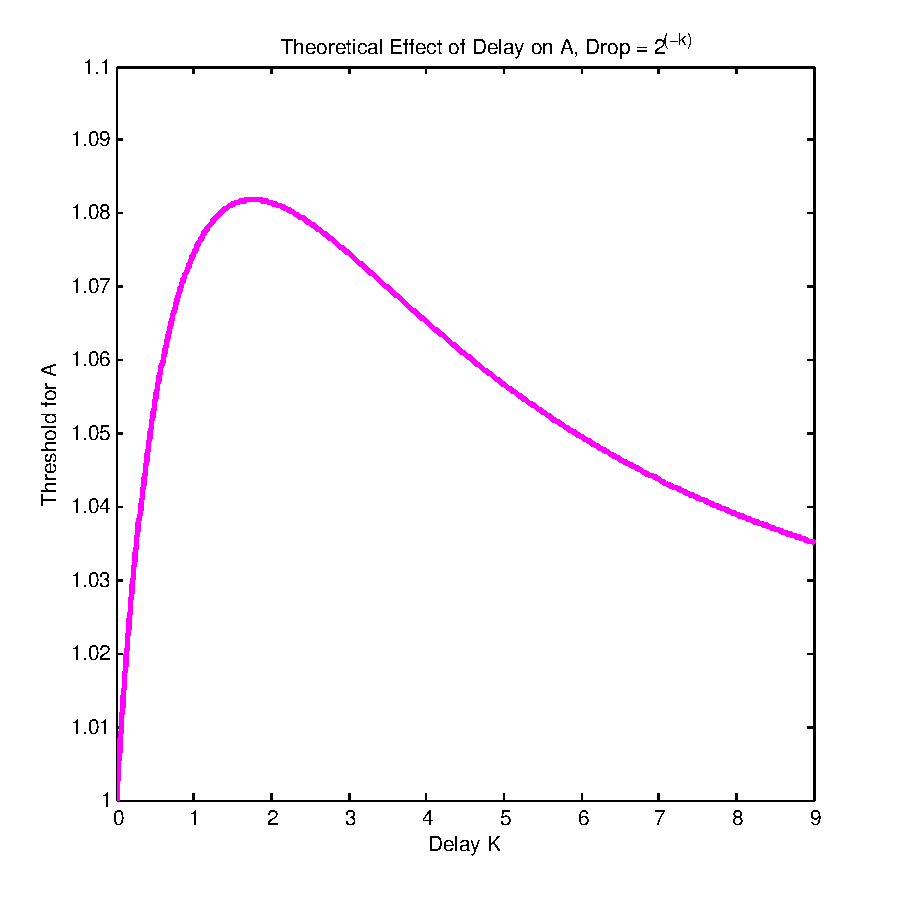
\includegraphics[width=0.5\textwidth]{summer_theoretical}
\end{center}

\subsection{Model of 2015-03-04:}
\[ X(n+1) = AX(n) + W(n) + U(n) \]
\[ X(0) \sim N(0, 1) \]
\[ Y(n) = \gamma^p [ Q(x(n)) + v(n)] = \gamma^p [ c(n)x(n) + v(n) ] \]
\[ C(n) \sim N(1, 2^{-2R}) \]
\[ \gamma^p = Ber(1 - 2^{-(msg-R)}) \]
\textbf{Note}: $\gamma^p$ = probability makes it through and is successfully decoded\\

\textbf{Current parameters}:
\begin{itemize}
\item $R = \alpha * msg$ = number of bits of information in code
\item D delay
\item $\beta$ = rate of information through channel
\end{itemize}

We can recreate the summer plot by setting $\beta = 1$ and $\alpha = 0 \rightarrow R = 0$. This essentially means we need to drop the entire packet (all bits) for it to count as a drop. In the new plot, we have less we can drop because we want to make sure the information can be decoded, so we can only drop redundant bits.

\begin{center}
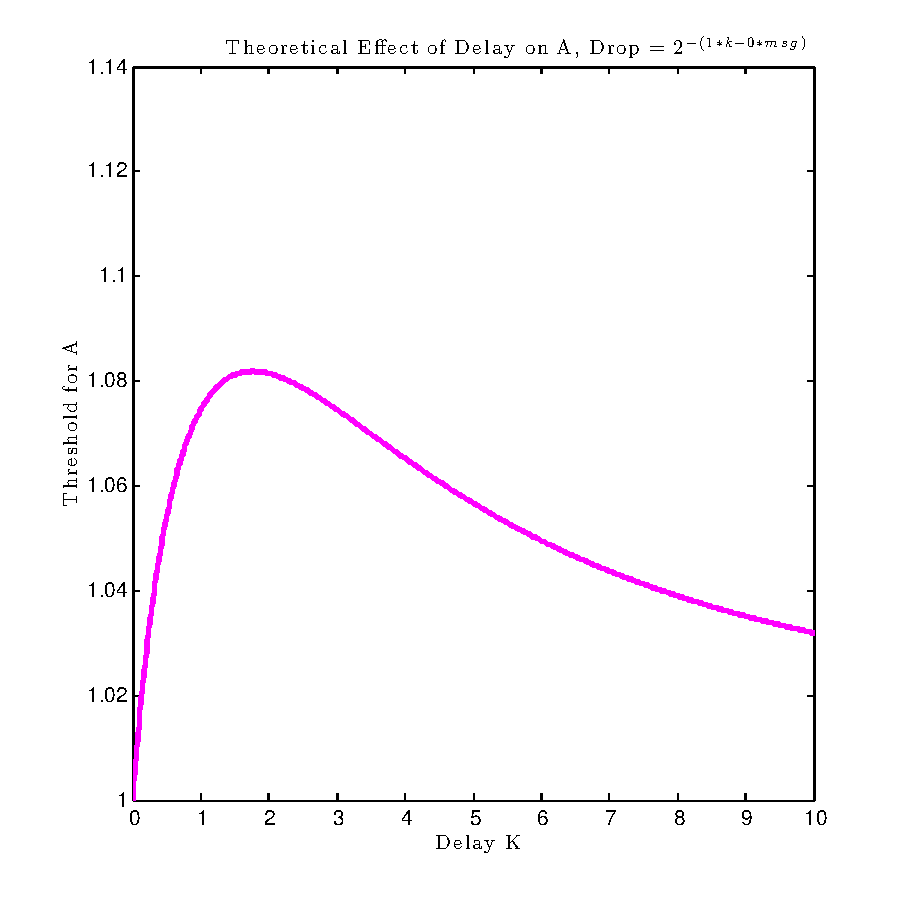
\includegraphics[width=0.5\textwidth]{newcode_oldplot}
\end{center}

\textbf{Note}: If R = msg, that is we don't send any redundancy, we automatically guarantee our packet will be dropped!!

\section{Empirical Support of Theoretical Curves}

\end{document}